%%%%%%%% MLSys 2027 submission: exact low-rank energy crossovers %%%%%%%%
% Anonymized research-track submission. Every number in this file traces to a
% committed run directory (results/analysis.json, results/summary.json) and a
% LOGBOOK.md entry in the repository; see the artifact statement.
%
% The \aslot macro marked A100 slots during drafting; none remain (2026-10-30).

\documentclass{article}

\usepackage{microtype}
\usepackage{graphicx}
\usepackage{booktabs}
\usepackage{amsmath,amssymb}
\usepackage{xcolor}
\usepackage{multirow}
\usepackage{array}
\usepackage{hyperref}

\newcommand{\theHalgorithm}{\arabic{algorithm}}

% Blind version for review. Switch to \usepackage[accepted]{mlsys2025} for camera-ready.
\usepackage{mlsys2025}

\mlsystitlerunning{When FLOPs Point the Wrong Way: Pre-Registered Energy Crossovers for Low-Rank Inference}

% ---- helpers ----
\newcommand{\aslot}[1]{\textcolor{red}{[A100: #1]}}
\newcommand{\rstar}{r^{*}}
\newcommand{\Efact}{E_{\mathrm{fact}}}
\newcommand{\Edense}{E_{\mathrm{dense}}}
\newcommand{\us}{\,\mu\mathrm{s}}

\begin{document}

\twocolumn[
\mlsystitle{When FLOPs Point the Wrong Way: Pre-Registered Energy Crossovers for Low-Rank Inference on GPUs}

\mlsyssetsymbol{equal}{*}

\begin{mlsysauthorlist}
\mlsysauthor{Anonymous Authors}{anon}
\end{mlsysauthorlist}

\mlsysaffiliation{anon}{Anonymous Institution, Anonymous City, Anonymous Country}

\mlsyscorrespondingauthor{Anonymous Author}{anon.email@example.com}

\mlsyskeywords{energy measurement, GPU energy, FLOPs, low-rank factorization, dispatch overhead, pre-registration, roofline}

\vskip 0.3in

\begin{abstract}
A linear map of exact rank $r$ can be executed as one dense GEMM or as two thin GEMMs through a rank-$r$ intermediate, and operation counting says the factorized form saves energy exactly when $r < d/2$, for every batch size. We measure where that crossover actually falls on a consumer laptop GPU (RTX 4090 Laptop, 175 W cap) and on a data-center A100, over 224 shape, rank, and batch configurations per platform (1344 windows of 20 s each), after an instrumentation gate found that the NVML cumulative energy counter reports about 500 W-equivalent while the laptop GPU idles at 4 W yet agrees with integrated power within 1 percent on the A100, so the energy source is qualified per platform rather than assumed. At batch size one the measured crossover rank is 0.021$d$, 0.198$d$, 0.461$d$, and 0.497$d$ for $d = 512$ to 4096 on the laptop: the FLOPs rule is wrong by a factor of 24 where the dense matrix-vector product is dispatch bound and right where it is memory bound, with the transition set by the launch floor and the memory bandwidth, and on the A100 the library's kernel selection sets the same boundary. An additive model with three physical terms (multiply-accumulates, memory words, GPU commands) calibrated on two shapes predicts held-out energy with 12.4 and 8.1 percent median error on the two platforms (FLOPs: 59.6 and 45.0 percent) and makes fewer wrong realization choices, with coefficients that equal each device's power divided by its FP32 throughput. The hypothesis registered before the first run was refuted by the data and restated, and seven quantitative predictions for the A100 were filed with a commit hash before that platform was measured: three held (the registered thresholds on the crossover, the transition size, the validity of the counter) and four did not, including a per-MAC energy four times the filed range, and the paper reports why. All code, configurations, raw samples, and the pre-registration trail are released.
\end{abstract}
]

\printAffiliationsAndNotice{}

\section{Introduction}
\label{sec:intro}

Energy is the quantity data centers pay for and the quantity that FLOPs are supposed to stand in for. Nearly every published estimate of the energy of a machine learning workload, from model cards to carbon calculators to the efficiency arguments behind pruning, factorization, and quantization, uses the count of multiply-accumulate operations (MACs or FLOPs) as the proxy \cite{henderson2020systematic,schwartz2020green,patterson2021carbon,lacoste2019quantifying}. The proxy is convenient because it is a property of the algorithm alone. It is also, as a matter of physics, incomplete: the energy a GPU draws is set by which transistors switch, how many bytes cross the memory hierarchy, and how long the device sits at a floor power waiting for the host to issue the next command. None of these are visible to an operation count \cite{horowitz2014}.

The gap matters most where a systems designer has a choice between two realizations of the same function. This paper studies the simplest such choice that is common in inference systems. A linear map $y = Wx$ with $W = VU$ of exact rank $r$ (with $V$ of size $d \times r$ and $U$ of size $r \times d$) can be executed as one dense GEMM of $B d^2$ MACs or as two GEMMs of $2 B r d$ MACs through a $B \times r$ intermediate. Low-rank structure of this kind is the basis of factorized layers in speech and vision models \cite{sainath2013lowrank,denton2014exploiting,jaderberg2014speeding}, of adapters \cite{hu2022lora}, and of the compressed projections that inference engines apply to attention and feed-forward blocks. The FLOPs rule for the choice is one line: factorize when $r < d/2$, for every batch size $B$ and every map size $d$.

That rule is testable without any modeling assumption, because the two realizations compute the same function to floating-point tolerance, so the only thing that differs between them is energy. We built a measurement stack to test it, and the experiment was designed as a pre-registered study: hypotheses, analysis code, pass or fail criteria, and the calibration versus held-out split were committed before the first full run, the development platform's results refuted the hypothesis as registered, the hypothesis was restated with the missing variable, and seven quantitative predictions for a second, held-out platform were filed with a commit hash before that platform was measured. We report every step, including the two that went wrong.

\paragraph{Findings.} On the laptop GPU at $B = 1$ the measured crossover rank is $0.021d$ at $d = 512$, $0.198d$ at 1024, $0.461d$ at 2048, and $0.497d$ at 4096 (Figure~\ref{fig:crossover}, top): the FLOPs rule ($\rstar = d/2$) is wrong by a factor of 24 at the smallest size and right at the largest. The reason is a change of regime, not of arithmetic. A $512 \times 512$ matrix-vector product takes 14.0$\us$ at 64 W, which is the host's launch floor at a reduced clock, and the factorized form with two launches takes 1.8 times as long at half the power, so it saves nothing however small $r$ is; at $d = 4096$ the dense product streams 64 MB at 520 GB/s, bytes scale with MACs, and the rule holds. The transition sits at $d_t = \sqrt{t_{\mathrm{launch}}\,\mathrm{BW} / 4\ \mathrm{B}}$, about 1360 on this platform and 1880 on the A100. An additive model with three physical terms, calibrated by non-negative least squares on $d \in \{512, 2048\}$ and scored once on $d \in \{1024, 4096\}$, predicts held-out energy with 12.4 percent median error on the laptop and 8.1 percent on the A100 (FLOPs: 59.6 and 45.0 percent), with coefficients that read as physics: 15.3 and 40.0 pJ per MAC, which on both devices is the power divided by the FP32 throughput. None of this is reportable without knowing what the sensor measures: the NVML energy counter, the quantity that most GPU energy tools read, advances at about 500 W-equivalent while the laptop GPU idles at 4 W, and agrees with integrated power within 1 percent on the A100, so the energy source is qualified per platform by pre-registered criteria.

\paragraph{Contributions.}
\begin{enumerate}
\item An exact-pair design for energy crossovers with a calibrate-then-predict protocol and pre-registered criteria, and a 1344-window dataset per platform of per-call energy, time, power, clock, temperature, and command counts for dense and factorized realizations of the same maps (Section~\ref{sec:design}).
\item The measured crossover map $\rstar(B, d)$ on two GPUs and its mechanism: a dispatch- or latency-bound regime at floor power, a memory-bound regime where the FLOPs rule holds, a compute-bound regime at the cap, with the transition size set by launch time and bandwidth and, on the A100, by the library's kernel selection (Sections~\ref{sec:results} and \ref{sec:a100}).
\item A three-term additive energy model that predicts held-out energy and realization choices from a two-shape calibration, against FLOPs and against a max-of-times model with regime power (Section~\ref{sec:models}).
\item A ten-criterion measurement gate that qualifies the energy source per platform, and the finding that the NVML energy counter is not the GPU's energy on one of two platforms (Section~\ref{sec:measurement}); and a pre-registration trail with two refutations and seven predictions scored as filed (Section~\ref{sec:a100}).
\end{enumerate}

What the paper does not claim: nothing here is about model quality, since the two realizations compute the same function to $10^{-4}$ relative Frobenius error and every claim is about energy per executed call; and the coefficients are calibrated per device, so the claim is that a model with these three terms, calibrated on a handful of shapes, predicts the rest of the grid, and that FLOPs does not.

\section{Energy accounting beyond operation counts}
\label{sec:background}

\paragraph{Three physical terms.} The accounting follows the transistor-operations framework of \citet{syed2026toml}, which assigns every arithmetic operation, every memory word moved between levels, and every dispatched GPU command a cost proportional to the transistor switching events it causes. With one arithmetic type here (FP32 multiply-accumulate) the model is

\begin{equation}
E_{\mathrm{M1}} = a_c\, N_{\mathrm{MAC}} + a_m\, N_{\mathrm{HBM}} + a_o\, S_o,
\label{eq:m1}
\end{equation}

where $N_{\mathrm{MAC}} = B d^2$ (dense) or $2 B r d$ (factorized); $N_{\mathrm{HBM}}$ counts every operand read or written once per call ($X$, the weights, the intermediate written and read back, $Y$) in 4-byte words; and $S_o$ is the number of GPU commands per call (kernel launches, copies, memsets), measured by a profiler where possible. The coefficients $a_c$, $a_m$, $a_o \geq 0$ are fitted per device by non-negative least squares. A variant M2 charges weights whose cycled footprint fits in L2 at an SRAM cost; with the cache-defeating protocol below this touches only factorized weights at small $r$. The FLOPs baseline P0 is $E = k\, N_{\mathrm{MAC}}$ with one fitted $k$, and it predicts $\rstar = d/2$ for every $B$ and $d$. With a single operation type the ratios in the published cost table do not enter the fit, so this experiment tests a three-term physical model against FLOPs, not the table itself.

\paragraph{Why the additive form can fail.} Equation~\ref{eq:m1} charges each command a fixed energy, but a command that cannot be overlapped costs \emph{time} at whatever power the device draws while it waits, and that power depends on the clock the driver chooses. We therefore also register a max-of-times model M3 with regime power,

\begin{align}
t &= \max\!\left(S_o\, t_{\mathrm{launch}},\ \tfrac{\mathrm{bytes}}{\mathrm{BW}},\ \tfrac{N_{\mathrm{MAC}}}{R}\right), \nonumber \\
E_{\mathrm{M3}} &= p_{\mathrm{floor}}\, t + (p_{\mathrm{active}} - p_{\mathrm{floor}})\, t_{\mathrm{active}},
\label{eq:m3}
\end{align}

with $p_{\mathrm{active}}$ equal to $p_{\mathrm{compute}}$ where the compute time dominates and $p_{\mathrm{memory}}$ otherwise, fitted jointly on energy and per-call time. M3 is the energy roofline of \citet{choi2013roofline} with a launch floor added.

\paragraph{The transition size.} At $B = 1$ the dense realization is one GEMV whose time is the larger of the launch floor $t_{\mathrm{launch}}$ and the time to stream $4 d^2$ bytes at bandwidth BW. The two are equal at

\begin{equation}
d_t = \sqrt{t_{\mathrm{launch}}\, \mathrm{BW} / 4\ \mathrm{B}}.
\label{eq:dt}
\end{equation}

Below $d_t$ the dense call is dispatch bound and a second launch is pure loss; above it the call is memory bound, bytes scale with MACs, and the FLOPs rule is right. Equation~\ref{eq:dt} is the formula from which the cross-platform predictions in Section~\ref{sec:a100} were derived.

\section{Measurement: qualifying the energy source}
\label{sec:measurement}

\paragraph{Platforms.} Two platforms as different as two CUDA devices can be, running the same pinned stack (Python 3.12, PyTorch 2.6.0 with CUDA 12.4, cuDNN 9.1, nvidia-ml-py 13.595.45): a laptop with an RTX 4090 Laptop GPU on Windows 11 (driver 595.79), 175 W enforced limit, 64 MiB L2, display on the integrated GPU; and a Linux SLURM node (driver 580.173.02) with four A100-SXM4-40GB, 400 W limit, 40 MiB L2, of which the job uses one with the whole node allocated. The laptop is where the protocol and the model were developed and calibrated; the A100 was measured only after every prediction for it had been filed.

\paragraph{Two energy quantities.} NVML exposes an instantaneous power reading (the \texttt{PowerUsage} query) and a cumulative energy counter (the \texttt{TotalEnergyConsumption} query, in mJ). Most GPU energy tools read one or the other \cite{you2023zeus,anthony2020carbontracker,lacoste2019quantifying}. Both are recorded in every measured window: the counter delta at CUDA-synchronized boundaries, and the trapezoid integral of the power reading sampled every 50 ms. Which one is \emph{the} energy is decided per platform by the gate below, and the other is kept as a same-sensor consistency check, never as independent validation.

\paragraph{The gate.} Before any science on a platform, a 20-minute instrumentation run evaluates ten pre-registered criteria (Table~\ref{tab:gate}) on a compute-bound FP32 $4096 \times 4096$ GEMM and a dispatch-bound loop of $64 \times 64$ GEMMs: counter support, monotonicity, update period, and agreement with the integral over ten 10 s blocks; repeatability across blocks; thermal settling after a 60 s heat load; the smallest window length with CV at or below 2 percent for it and all longer lengths; isolation from foreign processes; forbidden throttle reasons; identity of the torch and NVML devices by UUID (they can diverge under SLURM's device remapping); and the fraction of power samples above a plausibility ceiling. C1 to C3 do not gate; they select the energy source: the counter if all three pass, the power integral otherwise.

\begin{table*}[t]
\caption{Instrumentation gate and its outcome on the two platforms. C1 to C3 select the energy source; C4 to C10 gate.}
\label{tab:gate}
\vskip 0.1in
\centering
\small
\begin{tabular}{@{}llll@{}}
\toprule
ID & Criterion (threshold) & Laptop & A100 \\
\midrule
C1 & counter supported, monotonic & pass & pass \\
C2 & counter update period ($\leq$ 200 ms) & 100 ms & 101 ms \\
C3 & counter vs integral, max $|$rel$|$ ($\leq$ 0.05) & \textbf{1.996} & 0.010 \\
C4 & CV energy/call, GEMM ($\leq$ 3\%), loop ($\leq$ 5\%) & 0.32\%, 1.99\% & 0.80\%, 1.10\% \\
C5 & thermal settle after heat load ($<$ 300 s) & 16 s & 14 s \\
C6 & foreign compute processes (0) & 0 & 0 \\
C7 & smallest sufficient window, GEMM ($\leq$ 10 s) & 0.5 s & 0.5 s \\
C8 & forbidden throttle reasons (none) & none & none \\
C9 & torch UUID = NVML UUID & true & true \\
C10 & implausible power samples ($\leq$ 1\%) & 0 / 14877 & 0 / 15436 \\
\midrule
 & energy source selected & integral & counter \\
\bottomrule
\end{tabular}
\end{table*}

\paragraph{What the gate found.} On the laptop the counter is supported, monotonic, and updates every 100 ms, and it is not the GPU's energy: it advanced by 26.0 kJ across a 55 s settled idle window during which the power reading was 4.4 W (242 J), that is, at about 500 W-equivalent on a 175 W part; under the 175 W-capped GEMM it reported 1.51 J per call against 1.01 J from the integral, and for the dispatch loop 2.9 mJ against 1.1 mJ. The ratio is not constant, so no calibration factor rescues it; the first power reading after NVML initialization was a 593.5 W glitch, which motivated the plausibility ceiling (C10). On the A100 the same counter agreed with the integral within 1.0 percent on every 10 s block and within 0.1 percent over the 55 s idle windows, with a 101 ms update period. The laptop's energy is therefore the power integral and the A100's is the counter; a tool reading the counter alone would have reported the laptop's idle energy wrong by two orders of magnitude.

\paragraph{Regimes seen at the gate.} Under the laptop's cap, energy per call is a timing measurement: power is pinned at 175 W and the 0.9 percent rise across ten blocks is thermal (the SM clock fell 22 MHz as the die reached 79 C). The dispatch-bound loop is the informative regime: block-to-block variation lives in the block duration (9.26 to 9.91 s for a fixed call count), power sits near 60 W, and 20 s windows are needed for 2 percent CV. On the A100 the launch floor is 9.9$\us$ per call at 116 W against 14 to 19$\us$ at 60 W on the laptop, so one tiny call costs nearly the same energy on both (1.16 against 1.11 mJ) by opposite routes; the A100 idles at 79 W. Temperature enters energy differently on the two: under the laptop's cap the clock falls at fixed power; on the A100 the clock holds at 1410 MHz and power rises from 393 to 399 W as the die warms from 64 to 69 C. Both are leakage; one shows up as time, the other as power.

\paragraph{Protocol after the gate.} Every measured window is 20 s, preceded by a 2 s warmup of the same configuration; before each shape's block sequence the GPU is settled under a mid-grid load until its temperature spread is at most 1 C over 5 s (a fixed 30 s warmup at 60 W does not reach steady state after a 175 W sequence); condition order within a shape is randomized with the run seed; the sampler runs at 50 ms; mean power, temperature, SM clock, and throttle reasons are recorded per window, with a regime label (\emph{capped} or \emph{uncapped}) from the fraction of samples reporting the software power cap.

\section{Experimental design and pre-registration}
\label{sec:design}

\paragraph{Workload.} The map sizes are $d = 512$, 1024, 2048, and 4096; the rank fractions $f = r/d$ are 1/64, 1/32, 1/16, 1/8, 1/4, 3/8, 1/2, and 3/4; the batch sizes are 1, 4, 16, 64, 256, 1024, and 4096. For each $(d, f)$, weights $V$ and $U$ are drawn with a fixed seed and $W = \mathrm{fp32}(\mathrm{fp64}(V)\,\mathrm{fp64}(U))$ is precomputed, so both realizations execute the same weight set on the same inputs. Everything is FP32 with TF32 disabled; outputs and intermediates are preallocated and the measured loop allocates nothing. To defeat the cache, $K = \lceil 2\,L2 / 4d^2 \rceil$ independent weight sets per shape are cycled call by call, so the dense footprint is at least twice the L2; factorized sets cycle identically. Exactness is verified for every configuration (maximum relative Frobenius difference $10^{-5}$ against a $10^{-4}$ exclusion tolerance; nothing was excluded). The grid is 224 configurations per platform, two realizations each, three randomized repetitions of 20 s windows: 1344 windows and 8.5 to 8.7 hours per platform.

\paragraph{Calibration and held-out split.} The shapes $d \in \{512, 2048\}$ are the calibration set and $d \in \{1024, 4096\}$ are held out. Model selection (M1 versus M2) uses leave-one-$(d, B)$-cell-out cross-validation over the 14 calibration cells only, scored by the mean over folds of the median absolute percentage error (APE), ties to M1. The held-out shapes are scored once by the analysis script; nobody tunes on them. Fits use relative weighting (rows scaled by $1/E$) so that the objective matches the percentage-error criteria.

\paragraph{Crossover estimation.} For each $(d, B)$ cell the measured crossover $\rstar$ is the rank at which the repetition-mean ratio $\Efact / \Edense$ crosses 1, by log-linear interpolation between tested ranks; a cell is \emph{dense always} if the ratio exceeds 1 at every tested rank. Predicted crossovers come from the selected model on the held-out shapes with two 95 percent bootstrap intervals per cell (1000 resamples each), one from resampling calibration windows (prediction uncertainty) and one from resampling the held-out repetitions (measurement uncertainty).

\paragraph{The registered hypothesis and criteria.} H2a, registered on 2026-09-15 before the first full run (commit tagged \texttt{exp-002-protocol}): at $B = 1$ the measured $\rstar$ is at most $d/4$ or dense wins throughout; $\rstar(B)$ is non-decreasing in $B$; the three-term model calibrated on two shapes predicts $\rstar(B)$ on the two held-out shapes; and FLOPs is wrong by at least a factor of 2 at $B = 1$. The criteria are in Table~\ref{tab:criteria}. Two dated amendments preceded any full-run data: the analysis code was written and tested on synthetic runs from a known three-term model while the laptop run was in progress, and E2 was amended from "measured $\rstar$ inside the prediction interval" to "the two intervals overlap", because a tight calibration fit gives a prediction interval 0.1 percent wide while the measured $\rstar$ carries 1 to 2 percent repetition noise, so even a model predicting $\rstar$ within 2 percent fails every cell. The point rule (same verdict kind and $\rstar$ within a factor of 1.5) is reported alongside and became the gating rule in v3.

\begin{table*}[t]
\caption{Pre-registered criteria for EXP-002 and their outcome: laptop under v2 (the run's frozen config) and A100 under v3 (frozen with the predictions; E2 gates on the point rule, E3 and E4 apply to $d = 1024$ with the E4 threshold 0.7, E8 and E10 gate). E6 and E9 are reported, not gating.}
\label{tab:criteria}
\vskip 0.1in
\centering
\footnotesize
\begin{tabular}{@{}lp{6.2cm}p{4.6cm}p{4.6cm}@{}}
\toprule
ID & Criterion (threshold) & Laptop (v2) & A100 (v3) \\
\midrule
E1 & held-out median APE of the selected model ($\leq 20\%$) & \textbf{pass}: M1, 12.4\% (FLOPs 59.6\%) & \textbf{pass}: M1, 8.1\% (FLOPs 45.0\%) \\
E2 & crossover coverage over 14 held-out cells ($\geq 12$) & \textbf{fail}: intervals overlap 3 of 14; point rule 13 of 14 & \textbf{fail}: point rule 11 of 14; intervals overlap 4 \\
E3 & $\rstar(B{=}1) \leq d/4$ or dense always, model on the same side & \textbf{fail}: 1024 pass (202 vs 206); 4096 fail (2034) & \textbf{fail}: 1024 measured 293, model dense always \\
E4 & $\rstar(B)$ non-decreasing in $B$, Spearman threshold & \textbf{fail}: 0.79 and $-0.04$ ($\geq 0.8$) & \textbf{fail}: 0.67 ($\geq 0.7$) \\
E5 & exactness exclusions ($\leq 5\%$) & \textbf{pass}: 0 of 224 & \textbf{pass}: 0 of 224 \\
E6 & summed regret over the held-out grid ($\leq 5\%$) & 0.06\% (FLOPs 0.09\%) & 0.92\% (FLOPs 0.95\%) \\
E7 & 0 contaminated windows, $\leq 1\%$ implausible samples & \textbf{pass}: 0, 0 & \textbf{pass}: 0, 0 \\
E8 & M3 point rule ($\geq 12$ of 14) & 11 of 14 (exploratory) & \textbf{fail}: 11 of 14 \\
E9 & M3 held-out median APE $\leq$ M1's & 24.0\% (reported) & 14.6\% (reported) \\
E10 & $\rstar(B{=}1)/d \leq 0.30$ at 1024 and $\geq 0.45$ at 4096 & 0.198, 0.497 (exploratory) & \textbf{pass}: 0.286, 0.496 \\
\bottomrule
\end{tabular}
\end{table*}

\paragraph{Timeline.} 2026-09-15: protocol, hypothesis, criteria, and configuration committed and tagged; laptop full run started at 18:07 local time. 2026-09-16 to 18: analysis; H2a refuted as stated; the restated H2a$'$, the v3 criteria, the M3 registration, and seven A100 predictions (Section~\ref{sec:a100}) committed and tagged \texttt{exp-002-a100-predictions}. 2026-09-25: A100 gate run. 2026-10-30: A100 EXP-002 run (00:12 to 08:40 cluster time) and its analysis, with the script and the v3 criteria as frozen at the prediction commit.

\section{Results on the development platform}
\label{sec:results}

\paragraph{Run quality.} The laptop run (\texttt{20260915T180708}) measured all 1344 windows (261 before an external kill at about 19:54, the rest after a resume from the crash-safe window ledger, with no window lost), 537,600 power samples with none above the plausibility ceiling, zero foreign processes, and zero exactness exclusions. The repetition CV of energy per call has median 0.76 percent, 90th percentile 4.7 percent, and maximum 15.8 percent, the large values confined to dispatch-bound cells where the host's timing is the noise. Dense energy at fixed $(d, B)$ varies by at most 2 percent across the eight weight sets of different rank, so the data dependence of GEMM energy is negligible here.

\paragraph{Three regimes.} Supplementary Figure 1 shows per-call time, mean power, and energy at $B = 1$ against $d$ for both realizations at $r/d = 1/16$. Dispatch bound ($d = 512$): the dense GEMV takes 14.0$\us$ at 64 W; the factorized form with two launches takes 25.4$\us$ at 33 W with the SM clock at 1455 MHz instead of 2325 MHz. Twice the launches, 1.8 times the time, half the power: the GPU downclocks while it waits for the host, so a launch's energy is not a constant, and at the smallest rank the two realizations cost the same within 2 percent. Memory bound ($d = 4096$): the dense GEMV reads 64 MB in 123$\us$ at 520 GB/s on a 576 GB/s part, at 149 W and uncapped, while the factorized form at $r/d = 1/16$ reads 8 times fewer weight bytes and costs 7 times less energy. Compute bound ($B = 4096$): every cell sits at the 175 W cap, time is proportional to MACs at 23.6 TFLOPS, and the factorized form at $f = 1/2$ costs 1.7 percent more than the dense form because its thinner GEMMs run at slightly lower throughput.

\paragraph{The crossover map.} Table~\ref{tab:crossovers} (left) and Figure~\ref{fig:crossover} (top) give the measured $\rstar/d$ for all 28 cells. At $B = 1$ the fraction rises with $d$: 0.021, 0.198, 0.461, 0.497. The FLOPs rule is wrong by a factor of 24 at $d = 512$, 2.5 at 1024, 1.1 at 2048, and 1.0 at 4096; at $d = 512$ and $B = 4$ dense wins at every tested rank. At fixed $d$ the fraction rises with $B$ where dispatch matters ($d \leq 1024$) and is flat near $d/2$ for $d \geq 2048$. Figure~\ref{fig:ratio} (left) shows the mechanism: at $B = 1$ the energy ratio for $d = 512$ is flat near 1 at every rank, $d = 4096$ follows the FLOPs line $2r/d$, and the intermediate sizes bend between the two; at $B = 4096$ (Supplementary Figure 2) all four sizes collapse onto the FLOPs line except for a 5 to 15 percent penalty at the largest ranks.

\begin{table*}[t]
\caption{Measured crossover rank $\rstar/d$ on the laptop GPU (left) and the A100 (right); rows $d$, columns $B$. The FLOPs rule predicts 0.5 in every cell; "dense" means dense wins at every tested rank.}
\label{tab:crossovers}
\vskip 0.1in
\centering
\small
\setlength{\tabcolsep}{3.5pt}
\begin{tabular}{@{}lrrrrrrrcrrrrrrr@{}}
\toprule
 & \multicolumn{7}{c}{Laptop} & & \multicolumn{7}{c}{A100} \\
\cmidrule{2-8} \cmidrule{10-16}
$d$ & 1 & 4 & 16 & 64 & 256 & 1024 & 4096 & & 1 & 4 & 16 & 64 & 256 & 1024 & 4096 \\
\midrule
512  & 0.021 & dense & 0.169 & 0.157 & 0.219 & 0.368 & 0.503 & & dense & dense & dense & dense & 0.228 & 0.446 & 0.468 \\
1024 & 0.198 & 0.366 & 0.262 & 0.327 & 0.336 & 0.443 & 0.473 & & 0.286 & dense & dense & 0.203 & 0.481 & 0.438 & 0.444 \\
2048 & 0.461 & 0.459 & 0.365 & 0.327 & 0.444 & 0.405 & 0.463 & & 0.157 & 0.334 & 0.307 & 0.378 & 0.403 & 0.523 & 0.521 \\
4096 & 0.497 & 0.421 & 0.466 & 0.538 & 0.415 & 0.467 & 0.491 & & 0.496 & 0.456 & 0.458 & 0.475 & 0.503 & 0.444 & 0.521 \\
\bottomrule
\end{tabular}
\end{table*}

\begin{figure*}[t]
\centering
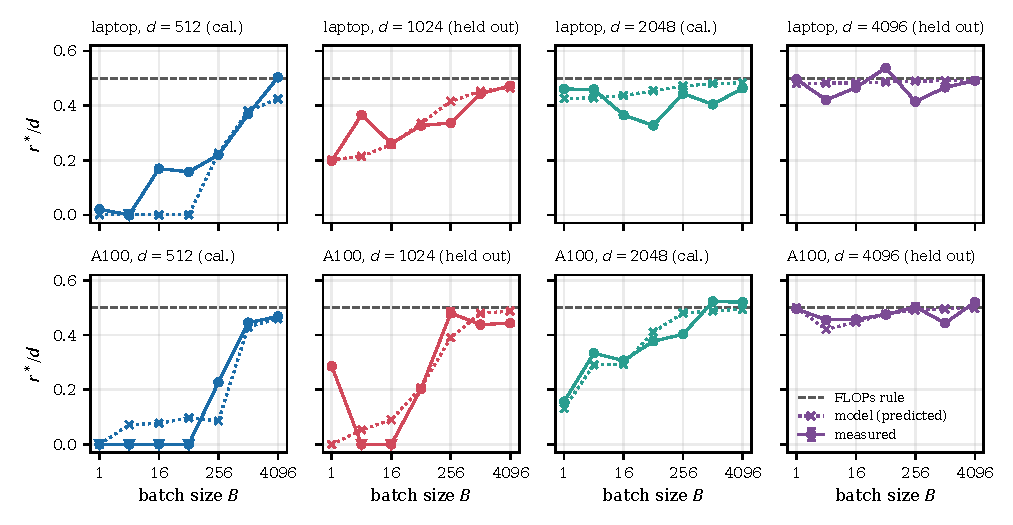
\includegraphics[width=\textwidth]{figures/crossover_map_both.pdf}
\caption{Measured crossover rank $\rstar/d$ against batch size on the laptop GPU (top) and the A100 (bottom): circles with 95 percent measurement intervals from resampled repetitions, triangles where dense wins at every tested rank, crosses for the additive model M1 (a fit on the calibration shapes $d = 512$ and 2048, a prediction on the held-out shapes $d = 1024$ and 4096), and the FLOPs rule (dashed). The rule is right only where the dense call is memory or compute bound.}
\label{fig:crossover}
\end{figure*}

\begin{figure*}[t]
\centering
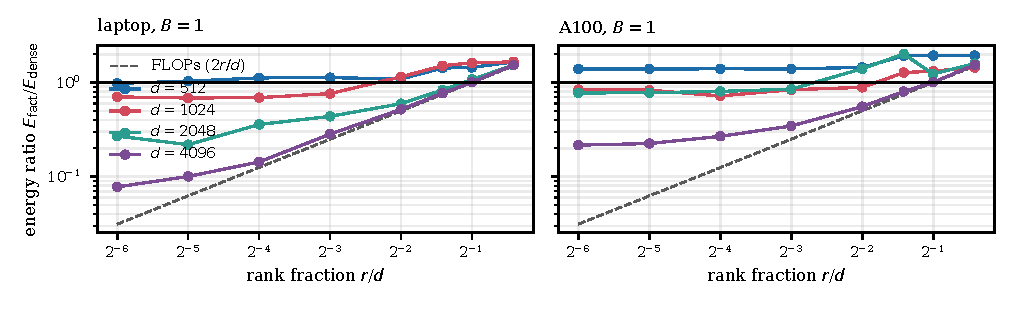
\includegraphics[width=\textwidth]{figures/ratio_b1_both.pdf}
\caption{Energy ratio $\Efact/\Edense$ against rank fraction at $B = 1$ on the laptop GPU (left) and the A100 (right); the FLOPs prediction is $2r/d$ (dashed). On the laptop the $d = 512$ ratio stays near 1 at every rank because both realizations sit on the launch floor. On the A100 the ratios follow cuBLAS's kernel selection: a constant 1.39 at $d = 512$, a jump at $d = 2048$ between $r/d = 1/8$ and $1/4$ where a four-kernel path is chosen, and a floor above the FLOPs line at $d = 4096$ until $r/d = 1/4$. The $B = 4096$ panels are in the supplement.}
\label{fig:ratio}
\end{figure*}

\paragraph{The registered hypothesis is refuted.} H2a fails on E2, E3, and E4 (Table~\ref{tab:criteria}). E3 fails on the measurement at $d = 4096$, where the $B = 1$ crossover is $0.497d$, not below $d/4$. E4 fails because monotonicity in $B$ holds only where dispatch matters (Spearman 0.79 at $d = 1024$, just under 0.8; $-0.04$ at $d = 4096$, where the curve is flat between 0.41 and 0.54 with repetition noise). E2 fails as an interval-overlap test: the measurement intervals are about 2 percent wide and the prediction intervals under 1 percent, so the test asks for exact agreement, which a model with 12 percent error cannot deliver while still making every decision correctly; under the point rule 13 of 14 cells agree within a factor of 1.5, the one miss being $(1024, 4)$ with measured $\rstar = 374$ against predicted 220. The hypothesis was mis-specified by leaving $d$ out, and we restated it as H2a$'$: $\rstar(B{=}1)/d$ rises with $d$ from far below 1/2 to about 1/2 across $d_t$; below $d_t$, $\rstar$ rises with $B$; well above $d_t$, $\rstar \approx d/2$ for every $B$; and the FLOPs error grows as $d$ falls below $d_t$. H2a$'$ was committed with the A100 predictions and tested only on the A100 (Section~\ref{sec:a100}).

\paragraph{A deviation that inverted the first analysis.} The command census, which runs \texttt{torch.profiler} with the CUDA activity on every configuration after five warmup calls, recorded no device events on this Windows machine and wrote 0 commands per call everywhere. The analysis as first executed on 2026-09-16 therefore fitted every model with a dispatch feature identically zero (held-out median APE 23.4 percent). The corrected analysis of 2026-09-18, from the unchanged run files, treats a non-positive census as unknown and uses the declared count of one command per GEMM (1 dense, 2 factorized), the protocol's registered fallback; both executions are in the repository, and every laptop number is labeled "command counts declared, not measured" in the logbook. On the Linux platform the census returned device events for every configuration: 1 to 4 commands per call (72, 206, 115, and 55 of the 448 configuration and realization pairs), with cuBLAS choosing a split-K matrix-vector kernel plus a reduction kernel for many dense $B = 1$ calls and up to four kernels for the factorized form, so the A100 analysis uses measured counts.

\section{Predicting energy and the right realization}
\label{sec:models}

\paragraph{Model selection and coefficients.} Cross-validation over the 14 calibration cells selects M1 (mean fold median APE 0.152 against 0.160 for M2, which differ only in the L2 charge on small factorized weights). The M1 coefficients on $d \in \{512, 2048\}$ are $a_o = 0.637$ mJ per command (95 percent bootstrap interval 0.632 to 0.642), $a_c = 15.3$ pJ per MAC (15.27 to 15.31), and $a_m = 1.03$ nJ per HBM word (1.024 to 1.033). The FLOPs model fits $k = 23.3$ pJ per MAC, that is, it absorbs memory and launch energy into a 50 percent inflated arithmetic cost and then misallocates it across the grid.

\paragraph{Held-out accuracy.} On the 672 held-out windows M1 reaches a median APE of 12.4 percent (90th percentile 26.1 percent, maximum 65.2 percent; calibration median 10.7 percent). P0 reaches 59.6 percent (Figure~\ref{fig:scatter}). M1's largest errors are the small-rank factorized cells at $B = 1$ (about 50 percent over), exactly the cells where the downclocked two-launch floor costs no more energy than one launch: an additive per-command energy cannot represent a cost that is paid in time at a power that depends on how idle the device has been, and the same failure recurs on the A100 (Section~\ref{sec:a100}). The FLOPs model's errors are structural: it under-predicts the dispatch-bound cells by up to a factor of 10 and over-predicts the memory-bound dense cells.

\begin{figure*}[t]
\centering
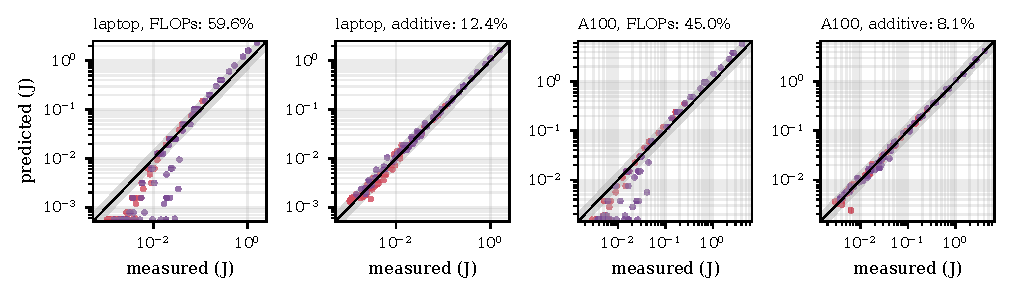
\includegraphics[width=\textwidth]{figures/heldout_scatter_row.pdf}
\caption{Predicted against measured energy per call on the held-out shapes ($d = 1024$ in red, 4096 in purple) for the FLOPs model and the additive model M1 on each platform, each calibrated on $d \in \{512, 2048\}$ of its own platform only; the band is a factor of 1.5 and the title gives the median error. FLOPs predictions below the axis range are drawn on its lower edge.}
\label{fig:scatter}
\end{figure*}

\paragraph{Decisions and regret.} For the system designer the question is which realization to choose. Over the 112 held-out $(d, f, B)$ cells, M1 picks the more expensive realization in 3 cells and FLOPs in 7. The registered regret (extra energy summed over the grid relative to the measured optimum) is 0.06 percent for M1 and 0.09 percent for FLOPs, dominated by the joule-scale cells where both rules are right; the per-cell relative regret, added as a reported metric after the run, averages 0.7 percent for M1 against 1.2 percent for FLOPs, with worst cells of 62 and 51 percent. The $B = 1$ crossovers are predicted within 3 percent on both held-out shapes (206 against 202 at $d = 1024$; 1972 against 2034 at $d = 4096$).

\paragraph{The max-of-times model.} M3, fitted jointly on energy and per-call time on the calibration shapes, yields $t_{\mathrm{launch}} = 16.6\us$, BW $= 443$ GB/s, 8.7 TMAC/s (17.4 TFLOPS), $p_{\mathrm{floor}} = 46$ W, $p_{\mathrm{memory}} = 175$ W, and $p_{\mathrm{compute}} = 184$ W. Its transition size from Equation~\ref{eq:dt} is $d_t = 1358$, between the two sizes where the measured $B = 1$ crossover jumps (0.198 at 1024, 0.461 at 2048), and it reproduces the $B = 1$ structure (0.174 and 0.500 on the held-out shapes against 0.198 and 0.497 measured). But it predicts energy worse than M1 (held-out median APE 24.0 percent, 11 of 14 cells under the point rule), because one throughput constant cannot represent cuBLAS's shape-dependent kernels, which run between 2 and 24 TFLOPS across the grid, and because its floor power is fixed while the real one moves with the clock. M3 explains the map; M1 predicts the numbers. M3 was fitted after the laptop data were seen and is exploratory here; it was registered as a secondary predictor for the A100 before that platform was measured.

\section{The held-out platform: predictions filed, then tested}
\label{sec:a100}

Seven predictions for the A100 were committed on 2026-09-18 (tag \texttt{exp-002-a100-predictions}) before any EXP-002 measurement on that platform. Their basis was the mechanism above, the A100's published HBM2e bandwidth (1555 GB/s) and FP32 throughput (19.5 TFLOPS), and the expectation of a launch floor of 5 to 20$\us$ on a Linux node, which the A100 gate later measured at 9.9$\us$. Each is falsifiable by the A100 run alone. Table~\ref{tab:a100} lists them with the outcome: three held and four did not.

\begin{table*}[t]
\caption{Predictions for the A100 filed before it was measured (tag \texttt{exp-002-a100-predictions}, 2026-09-18) and the outcome of run \texttt{20261030T001246}.}
\label{tab:a100}
\vskip 0.1in
\centering
\small
\begin{tabular}{@{}lp{5.9cm}p{5.9cm}p{2.3cm}@{}}
\toprule
ID & Prediction & Observed & Verdict \\
\midrule
A1 & $\rstar(B{=}1)/d$ rises with $d$: at most 0.30 at $d = 1024$ and at least 0.45 at $d = 4096$ & 0.286 at 1024, 0.496 at 4096; but the column is dense always, 0.286, 0.157, 0.496, so it does not rise monotonically & held as registered; monotone form fails at 2048 \\
A2 & $d_t$ between 1400 and 2800 (launch floor 5 to 20$\us$ at 1555 GB/s); hence $\rstar/d < 0.40$ at $(2048, 1)$ and $\geq 0.45$ at $(4096, 1)$ & M3 fit $d_t = 1883$; 0.157 at $(2048, 1)$; 0.496 at $(4096, 1)$ & held \\
A3 & at $B = 4096$ every shape's $\rstar/d$ between 0.42 and 0.50 & 0.468, 0.444, 0.521, 0.521: at $d \geq 2048$ the factorized form at $r = d/2$ costs 4 to 5 percent less than the dense form & failed \\
A4 & FLOPs wrong by $\geq 10\times$ at $(512, 1)$ or dense always; $\geq 2\times$ at $(1024, 1)$; $\leq 1.2\times$ at $(4096, 1)$ & dense always at 512; $1.75\times$ at 1024; $1.01\times$ at 4096 & failed (middle clause) \\
A5 & M1 coefficients: 0.5 to 2.0 mJ per command; 5 to 10 pJ per MAC; 0.3 to 1.0 nJ per HBM word & 1.17 mJ; 40.0 pJ; 0.74 nJ & failed (MAC term) \\
A6 & M1 held-out median APE $\leq 20\%$ and $\geq 12$ of 14 cells within a factor of 1.5 & 8.1\%; 11 of 14 & failed (coverage) \\
A7 & the A100's energy counter passes C1 to C3 and becomes its energy source & C3 0.010; counter selected; within 0.6\% of the integral in all 1344 windows & held \\
\bottomrule
\end{tabular}
\end{table*}

\paragraph{The run.} Run \texttt{20261030T001246} on one A100 of a whole-node SLURM allocation, at a clean tree, 8.5 hours, all 1344 windows in one session, 538,803 power samples with none above the plausibility ceiling, zero foreign processes, zero exactness exclusions; 80, 20, 5, and 2 weight sets cycled against the device's 40 MiB L2. The energy source was the counter, within 0.6 percent of the power integral in every window (median 0.2 percent). The repetition CV of energy per call has median 1.1 percent, 90th percentile 2.0 percent, and maximum 4.3 percent; dense energy varies by at most 4.9 percent across weight sets at fixed $(d, B)$; 93 windows ran at the 400 W cap, all large-batch GEMMs at $d = 2048$.

\paragraph{The crossover map.} Table~\ref{tab:crossovers} (right) and Figure~\ref{fig:crossover} (bottom) give the measured $\rstar/d$. At $B = 1$ the column reads dense always at $d = 512$, 0.286 at 1024, 0.157 at 2048, and 0.496 at 4096: the FLOPs rule is wrong by a factor of 1.75 at 1024, 3.2 at 2048, and right at 4096, and at 512 no rank saves energy. The two registered thresholds of A1 hold, but the column does not rise monotonically, and Figure~\ref{fig:ratio} (right) shows why. At $d = 512$ the ratio is 1.39 at every rank: cuBLAS runs the dense call as one matrix-vector kernel (25.9$\us$ at 82 W, well above the gate's 9.9$\us$ launch floor, so the kernel's own latency is the floor) and the factorized call as two (38.7$\us$ at 77 W). At $d = 1024$ the dense call becomes a split-K kernel plus a reduction (two commands, 30.8$\us$ at 130 W, 4.0 mJ) while the factorized call at small ranks runs three kernels at the floor power (2.9 to 3.4 mJ) and is 16 to 28 percent cheaper, so the crossover sits at $0.286d$. At $d = 2048$ the dense call is one memory-bound kernel (16.8$\us$ at 262 W, 1.0 TB/s, 4.4 mJ); the factorized call costs 3.4 to 3.7 mJ in three kernels for $r/d \leq 1/8$, jumps to 6.1 and 8.8 mJ at $r/d = 1/4$ and $3/8$ where cuBLAS selects a four-kernel path (60.8$\us$ at 101 to 145 W), and falls back to 5.4 mJ in two kernels at $r/d = 1/2$; the interpolated crossover, $0.157d$, marks a kernel-selection boundary rather than a byte count. At $d = 4096$ the dense call streams 64 MB in 58.5$\us$ at 287 W (16.7 mJ) and the factorized call at $r/d = 1/16$ costs 4.5 mJ at the floor power, a ratio of 0.27 against the FLOPs value of 0.125, until the ratio meets the FLOPs line at $r/d = 1/4$ and the crossover lands at $0.496d$. At $B = 4096$ all four sizes follow the FLOPs line, and at $d \geq 2048$ the kernel-shape penalty has the opposite sign from the laptop's: the two half-width GEMMs at $r = d/2$ cost 4 to 5 percent less than the dense GEMM, because the dense $2048^3$ kernel runs at the 400 W cap at 8.6 TFLOPS while the thinner ones run slightly faster, and at $d = 4096$ the dense product reaches 19.0 TFLOPS at 381 W while the thinner ones draw 353 W. That is the failure of A3, and it is a statement about cuBLAS, not about bytes.

\paragraph{Criteria and the restated hypothesis.} Under the v3 criteria frozen with the predictions (Table~\ref{tab:criteria}), E1, E5, E7, and E10 pass; E2 fails with 11 of 14 held-out cells under the point rule, the three misses being $(1024, 1)$, $(1024, 4)$, and $(1024, 16)$, where the model predicts dense always for the first and a numeric crossover for the other two and the measurement says the opposite in each case; E3 fails because the measured $\rstar(B{=}1)$ at $d = 1024$ is $0.286d$, above $d/4$, while the model predicts dense always; E4 fails with Spearman 0.67 against 0.7; and E8 fails with 11 of 14 for M3. H2a$'$ is therefore not supported on the A100 under the gate it was registered with. What survives the test is the structure the hypothesis was built on: the FLOPs rule fails at small $d$ and holds at large $d$ and large $B$, the transition size from Equation~\ref{eq:dt} lands where it was predicted to, and the additive model predicts the held-out grid better on this platform than on the one it was developed on. What does not survive is the claim that the $B = 1$ crossover is a smooth function of $d$ with the dispatch floor as the only small-size mechanism: on the A100 the library's choice of kernel at each shape sets the floor, the power, and the command count, and the map inherits its discontinuities. We did not amend any criterion after seeing the A100 data, and we do not re-score the failed predictions under alternative rules.

\paragraph{Predicting energy with measured command counts.} M1 is selected over M2 (cross-validation 0.121 against 0.123). Its coefficients on $d \in \{512, 2048\}$ are $a_o = 1.17$ mJ per command (1.168 to 1.173), $a_c = 40.0$ pJ per MAC (39.9 to 40.1), and $a_m = 0.741$ nJ per HBM word (0.738 to 0.744); the FLOPs model fits 55.7 pJ per MAC. Held-out median APE is 8.1 percent (90th percentile 21.3, maximum 62.7, calibration median 9.5) against 45.0 percent for FLOPs (90th percentile 98.4), Figure~\ref{fig:scatter} (bottom). The worst M1 cells are again the small-rank factorized calls at $B = 4$ and $B = 16$ for $d = 1024$ (62 percent over), where three or four kernels run at the floor power for less energy than three or four times the per-command coefficient. Choosing by M1 picks the more expensive realization in 12 of 112 held-out cells against 17 for FLOPs; the per-cell relative regret averages 3.9 percent against 5.2 percent, with the same worst cell at 88 percent for both (a $d = 1024$ cell where both rules factorize and the four-kernel path makes that the wrong call); the summed regret is 0.92 against 0.95 percent. M3, fitted on the calibration shapes, gives $t_{\mathrm{launch}} = 13.2\us$, BW $= 1071$ GB/s (69 percent of the published 1555), 7.4 TMAC/s (14.7 TFLOPS, 76 percent of peak), $p_{\mathrm{floor}} = 101$ W, $p_{\mathrm{memory}} = 362$ W, and $p_{\mathrm{compute}} = 364$ W, hence $d_t = 1883$; its held-out median APE is 14.6 percent with 11 of 14 cells under the point rule, so on this platform too the max-of-times model explains the map and the additive model predicts the numbers.

\paragraph{Why A5 failed, and what the coefficients say across platforms.} The filed range of 5 to 10 pJ per MAC assumed that the data-center part would be more efficient per FP32 multiply-accumulate than the laptop part. The datasheet says otherwise: 19.5 TFLOPS at 400 W is 41 pJ per MAC, and the fit returns 40.0; the laptop's 23.6 TFLOPS at its 175 W cap is 14.8 pJ per MAC, and its fit returned 15.3. On both platforms the compute coefficient is, within 4 percent, the device's power divided by its FP32 throughput, which is what a physical model should return and what could have been computed before filing the prediction; the error was ours, and it is the kind of error pre-registration exists to expose. The command coefficient is 1.8 times larger on the A100 (1.17 against 0.64 mJ), consistent with its higher floor power (101 against 46 W in the M3 fits); the memory coefficient is 0.72 times the laptop's (0.74 against 1.03 nJ per word), consistent with HBM2e against GDDR6. Across the two platforms the energy of a tiny call is nearly equal, the energy of a MAC differs by 2.6 times, and the energy of a word by 1.4 times; a FLOPs count represents none of this, and three calibrated coefficients represent all of it.

\section{Discussion}
\label{sec:discussion}

\paragraph{What a systems designer should take from the map.} The rule "factorize when $r < d/2$" is correct where the arithmetic is the cost, the large-batch, large-map corner of inference. Where serving systems spend their time, at small batch, in decode steps, in per-request adapters, in the small projections of an already compressed model, the rule errs by a factor of 1.75 to 24 on our two platforms, and outright in the cells where no rank saves energy, always in the direction of wasting energy: it recommends a factorization that pays extra launches and saves nothing. Equation~\ref{eq:dt} is the skeleton of the map and its two inputs come from a 20-minute gate run; on the A100 the flesh on that skeleton is cuBLAS's kernel selection, which the measured command census captures and a FLOPs count cannot. Fusing the two thin GEMMs, or capturing them in a CUDA graph, moves $d_t$ down; the protocol here measures by how much.

\paragraph{Why a measurement gate.} The API that reports 500 W-equivalent at a 4 W idle is the one energy tools recommend because it is cheaper than a sampled power trace, and nothing in it signals that it is wrong: it is supported, monotonic, and regular. A study that trusted it would have reported the laptop's dispatch-bound energies 2.6 times too high and its idle energy 100 times too high. Any energy study should state which NVML quantity it used and the agreement between the two on its platform.

\paragraph{Pre-registration as a systems practice.} Registering the hypothesis cost one afternoon and changed the paper twice. H2a was wrong in a way we would not have noticed had we written it after the data, because the dependence on $d$ was invisible in a hypothesis stated in $B$ alone; H2a$'$ assumed a smooth floor where the library's kernel choice makes a jagged one; and A5 was wrong by a factor the datasheet already contained. The protocol also caught a silent instrumentation error (a census writing zeros) because the analysis was committed before the data. The registered criteria are reported as they stand, failures included, with the dated amendments; the reader can judge which results were predicted and which were explained.

\paragraph{Limitations.} (1) One operation type: the experiment tests a three-term physical model against FLOPs, not the relative costs of different arithmetic operations in the transistor-operation table. (2) Laptop command counts are declared (one per GEMM), not measured, because the profiler returned no device events on Windows, and the Nsight Systems cross-check the protocol requires has not been completed; the A100 census shows one to four commands per call, so the laptop's declared counts are a lower bound whose multiplicity its command coefficient absorbs. (3) Coefficients are calibrated per device; we claim transfer of the mechanism and of the protocol, not of the coefficients. (4) FP32 only, with TF32 off; tensor-core paths change the compute coefficient and may move the regime boundaries. (5) Inference only; the backward pass is a separately registered experiment. (6) Two platforms, one of each kind; the laptop's cap makes its compute-bound regime a timing measurement. (7) Thermal state is controlled by settling, not by cooling to a fixed temperature, so the energies carry the 1 to 2 percent drift the gate measured.

\section{Related work}
\label{sec:related}

Carbon and energy reporting for machine learning uses FLOPs, parameter counts, or hardware time as the primary quantity \cite{strubell2019energy,henderson2020systematic,schwartz2020green,patterson2021carbon,lacoste2019quantifying,luccioni2023bloom}, and inference energy trends have been analyzed in the same units \cite{desislavov2023trends}. \citet{sze2017efficient} and \citet{yang2017energy} argued from accelerator design that memory traffic, not arithmetic, dominates neural-network energy and that pruning by operation count and by energy diverge; our experiment measures that divergence for a factorization decision on commodity GPUs and adds a third term, dispatch, that accelerator energy models omit. The roofline model \cite{williams2009roofline} bounds time by the larger of compute and memory time and \citet{choi2013roofline} extended it to energy; our M3 is an energy roofline with a launch floor and regime-dependent power, M1 its additive counterpart, and $d_t$ the ridge point of a matrix-vector product with a launch floor. The accuracy and update behavior of NVIDIA's built-in power sensors have been examined on Kepler \cite{burtscher2014measuring} and on recent parts \cite{yang2023parttime,yang2024accurate}, and GPU power modeling is surveyed by \citet{bridges2016understanding}; tools such as Zeus \cite{you2023zeus} and Carbontracker \cite{anthony2020carbontracker} read NVML quantities as ground truth, and the counter finding here shows that the choice of quantity is platform dependent. Instruction-level and architectural GPU power models \cite{arafa2020verified,kandiah2021accelwattch} explain where energy goes inside a kernel; ours is coarser by design, so that it can be calibrated from a handful of windows on any device. Factorized layers were introduced for speech \cite{sainath2013lowrank} and vision \cite{denton2014exploiting,jaderberg2014speeding} and low-rank adapters \cite{hu2022lora} add two thin GEMMs to every adapted projection, all reasoning in MACs; our measurement gives the energy cost of the launches and thinner kernels these methods introduce. Pre-registration separates prediction from postdiction \cite{nosek2018preregistration} and is rare in systems research; the protocol here is an attempt to make an energy claim falsifiable in that sense.

\section{Conclusion}
\label{sec:conclusion}

For the simplest realization choice in inference, dense or factorized execution of the same low-rank map, the FLOPs rule is right where the arithmetic is the cost and wrong by a factor of 1.75 to 24, or wrong outright where no rank saves energy, wherever the launch floor, the memory traffic, or the library's kernel choice is the cost; a three-term physical model calibrated on two shapes predicts the rest of the grid within 12.4 and 8.1 percent on the two platforms, with coefficients that read as physics. Getting there required qualifying the sensor per platform, registering the hypothesis before the data, and accepting its refutation twice. The dataset, code, and pre-registration trail (anonymized repository linked in the supplementary material) are released so that the next crossover, dense against sparse, small batch against batched, GPU against CPU, can be measured alike.

\bibliography{refs}
\bibliographystyle{mlsys2025}

\section*{AI Usage Disclosure}
A large language model assistant (Claude, Anthropic) was used throughout this work under the authors' direction: to draft and revise the measurement, experiment, and analysis code and the figure scripts; to draft the logbook and decision entries from the authors' notes; to search the literature and retrieve bibliographic records; and to draft and edit the prose of this paper. The study design, the hypotheses, the pre-registered criteria and their amendments, the A100 predictions, every measurement, and the interpretation of the data are the authors' own. All measurements were executed by the authors on hardware under their control; no data were generated by an AI tool. Every reference was verified by the authors against its publisher or proceedings record, and every number in the paper was checked by the authors against the committed analysis output.

% Define \NOAPPENDIX (uncomment the line below) to build the 10-page body plus
% references for the submission; the appendix is then compiled separately from
% supplementary.tex.
% \def\NOAPPENDIX{1}
\ifdefined\NOAPPENDIX\else
% Appendix of the MLSys 2027 submission. Included by main.tex unless \NOAPPENDIX is
% defined, and compiled on its own by supplementary.tex for the separate upload.
\appendix
\section{Instrumentation gate details}
\label{app:gate}

Table~\ref{tab:gate_detail} lists the gate measurements behind Table 1 of the main paper. On the laptop the counter advanced by 26.0 kJ over the 55 s pre-heat idle window against 242 J from the integrated 4.4 W power reading, reported 1.514 J per call against 1.015 J for the capped GEMM blocks (CV 4.2 against 0.32 percent), and 2.89 mJ against 1.107 mJ for the dispatch loop. The window-sufficiency sweep (six lengths from 0.5 to 20 s, five randomized repetitions each) gave a smallest sufficient length of 0.5 s for the capped GEMM on both platforms (a timing measurement at a pinned power) and 20 s for the dispatch loop on the laptop; on the A100 no length met the 2 percent target for the dispatch loop because the sweep ran while the die cooled from the 395 W sequence (a 2.4 percent trend over 100 s), which is why every later window on both platforms is preceded by thermal settling under load.

\begin{table}[h]
\caption{Gate measurements on the two platforms (full runs \texttt{20260915T164645} and \texttt{20260925T064203}).}
\label{tab:gate_detail}
\vskip 0.1in
\centering
\footnotesize
\begin{tabular}{@{}p{3.3cm}p{2.3cm}p{2.3cm}@{}}
\toprule
Quantity & Laptop & A100 \\
\midrule
Power limit (enforced) & 175 W & 400 W \\
Idle power, pre-heat (55 s) & 4.40 W, drift $-0.62$ W/min & 79.1 W, drift $-2.2$ W/min \\
Hot-idle bias after settling & $+0.006$ W & $+0.88$ W \\
Heat load, 60 s & 171.7 W, 74 C max & 379.5 W, 66 C max \\
Thermal settle after heat load & 16 s & 14 s \\
Power reading update period & 500 ms & 103 ms (20 ms native) \\
Counter update period & 100 ms & 101 ms \\
Capped GEMM, 10 blocks & 1.015 J/call, CV 0.32\% & 2.853 J/call, CV 0.80\% \\
Dispatch loop, 10 blocks & 1.107 mJ/call, CV 1.99\% & 1.159 mJ/call, CV 1.10\% \\
Dispatch loop, time and power per call & 14 to 19$\us$, 60 W & 9.9$\us$, 116 W \\
SM clock under the loop & 2325 MHz & 1410 MHz \\
Windows, samples & 83, 14877 & 83, 15436 \\
\bottomrule
\end{tabular}
\end{table}

\section{Held-out crossover cells and model parameters}
\label{app:tables}

Table~\ref{tab:cells} lists the 14 held-out $(d, B)$ cells per platform with the measured crossover, the M1 prediction, and whether the point rule (same verdict kind and $\rstar$ within a factor of 1.5) is met. The M3 parameter vectors are, for the laptop: $t_{\mathrm{launch}} = 16.6\us$, BW $= 443$ GB/s, $R = 8.70$ TMAC/s, $p_{\mathrm{floor}} = 46.4$ W, $p_{\mathrm{memory}} = 174.6$ W, $p_{\mathrm{compute}} = 183.7$ W; for the A100: $t_{\mathrm{launch}} = 13.2\us$, BW $= 1071$ GB/s, $R = 7.37$ TMAC/s, $p_{\mathrm{floor}} = 100.8$ W, $p_{\mathrm{memory}} = 362.4$ W, $p_{\mathrm{compute}} = 364.5$ W. Both fits are joint on energy and per-call time with the powers ordered within the cap, from 54 starting points, selected by the lowest cost.

\begin{table}[h]
\caption{Held-out cells: measured $\rstar$, M1 prediction, point-rule outcome. "dense" means dense wins at every tested rank.}
\label{tab:cells}
\vskip 0.1in
\centering
\footnotesize
\setlength{\tabcolsep}{4pt}
\begin{tabular}{@{}lrrrcrrc@{}}
\toprule
 & \multicolumn{3}{c}{Laptop} & & \multicolumn{3}{c}{A100} \\
\cmidrule{2-4} \cmidrule{6-8}
$(d, B)$ & meas. & M1 & hit & & meas. & M1 & hit \\
\midrule
(1024, 1) & 202 & 206 & yes & & 293 & dense & no \\
(1024, 4) & 374 & 220 & no & & dense & 54 & no \\
(1024, 16) & 268 & 263 & yes & & dense & 92 & no \\
(1024, 64) & 335 & 343 & yes & & 208 & 212 & yes \\
(1024, 256) & 344 & 426 & yes & & 492 & 400 & yes \\
(1024, 1024) & 454 & 464 & yes & & 449 & 492 & yes \\
(1024, 4096) & 484 & 476 & yes & & 455 & 499 & yes \\
(4096, 1) & 2034 & 1972 & yes & & 2032 & 2048 & yes \\
(4096, 4) & 1723 & 1975 & yes & & 1868 & 1725 & yes \\
(4096, 16) & 1908 & 1978 & yes & & 1875 & 1834 & yes \\
(4096, 64) & 2203 & 1995 & yes & & 1947 & 1954 & yes \\
(4096, 256) & 1698 & 2007 & yes & & 2061 & 2013 & yes \\
(4096, 1024) & 1912 & 2011 & yes & & 1818 & 2032 & yes \\
(4096, 4096) & 2012 & 2015 & yes & & 2133 & 2038 & yes \\
\bottomrule
\end{tabular}
\end{table}

\section{Additional figures}
\label{app:figures}

\begin{figure}[h]
\centering
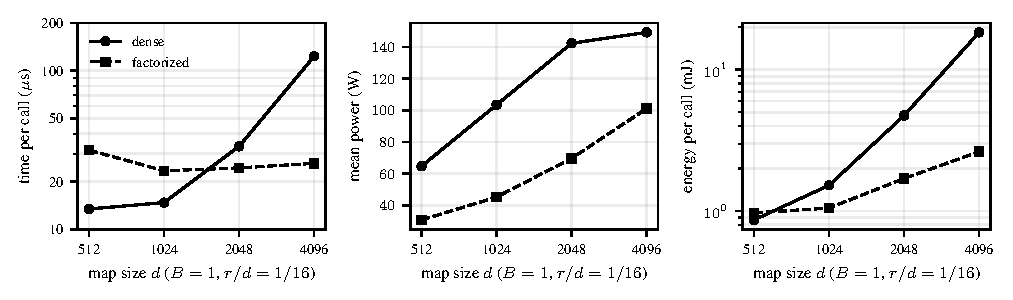
\includegraphics[width=\columnwidth]{figures/regimes_laptop.pdf}
\caption{Per-call time, mean power, and energy at $B = 1$ and $r/d = 1/16$ on the laptop GPU. The dense matrix-vector product sits on a 14$\us$ launch floor at reduced power up to $d \approx 1024$ and becomes memory bound above it; the factorized form pays two launches and saves energy only once the dense form is streaming weights.}
\label{fig:regimes}
\end{figure}

\begin{figure}[h]
\centering
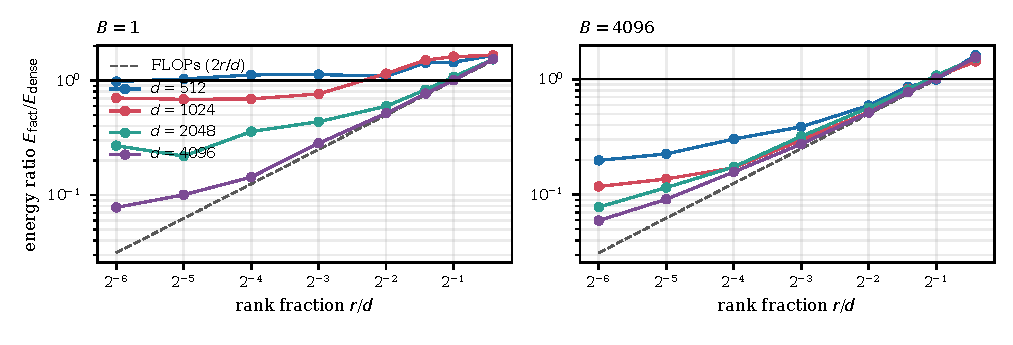
\includegraphics[width=\columnwidth]{figures/ratio_vs_rank_laptop.pdf}
\caption{Laptop GPU: energy ratio against rank fraction at $B = 1$ (left) and $B = 4096$ (right).}
\label{fig:ratio_laptop_full}
\end{figure}

\begin{figure}[h]
\centering
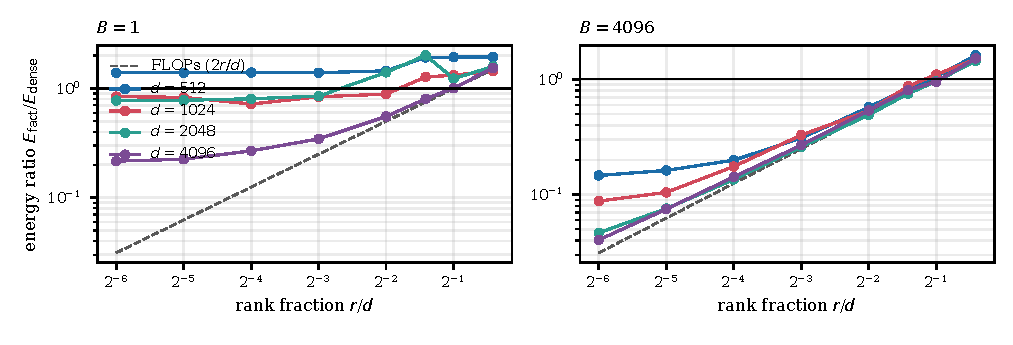
\includegraphics[width=\columnwidth]{figures/ratio_vs_rank_a100.pdf}
\caption{A100: energy ratio against rank fraction at $B = 1$ (left) and $B = 4096$ (right).}
\label{fig:ratio_a100_full}
\end{figure}

\begin{figure}[h]
\centering
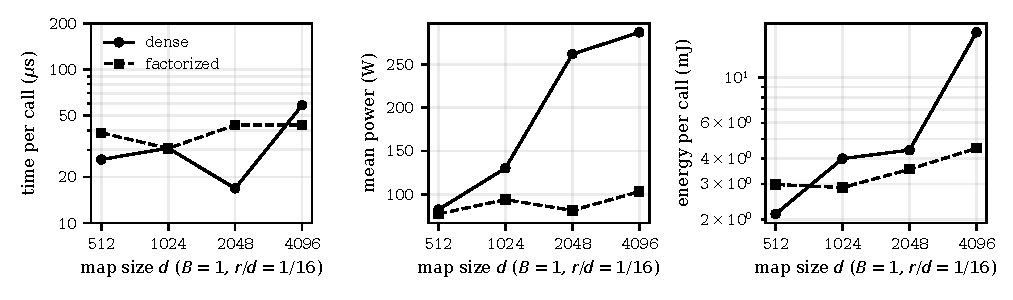
\includegraphics[width=\columnwidth]{figures/regimes_a100.pdf}
\caption{A100: per-call time, mean power, and energy at $B = 1$ and $r/d = 1/16$. Unlike the laptop (Figure~\ref{fig:regimes}), the dense call at $d = 2048$ is faster than at $d = 1024$ because cuBLAS switches from a split-K kernel plus a reduction to a single memory-bound kernel.}
\label{fig:regimes_a100}
\end{figure}

\fi

\end{document}

